\chapter{机器学习部分}
\label{chap:machinelearning}

\section{机器学习合理性论证}
\label{sec:threepone}
机器学习的核心是让计算机从已有数据中学习经验，理解其输入与输出之间的联系和规律，以使得计算机在处理新数据时能够预测未知信息。考虑本研究所面对的问题，中微子的运动学信息难以在实验中探测，若仅凭借其他信息就能对其复原，这几乎是不可思议的。因此，本研究在训练生成模型时所使用的数据实际上是利用蒙特卡洛方法得到的模拟数据，其中已预先包含中微子的动量信息作为扩散模型的部分输入。假设蒙特卡洛模拟数据与对撞机实验数据相比仅在整体上有系统性的偏离，那么对于对撞机实验数据，可以推测将其应用在训练完毕的生成模型上所得到的最终结果仍具有一定的合理性。受限于研究时限，在对撞机实验数据上的迁移过程尚未完成，所有关于机器学习结果的展示和比较均建立在原始的蒙特卡洛模拟数据基础上，具体可见第四章的结果部分。

本章将重点阐述所使用的机器学习方法的原理，以及基于此开发的OmniLearn生成模型的架构和它在$pp \to \tau \bar{\tau}$过程中的具体应用方式。
\section{扩散模型}
\label{sec:threeptwo}
\subsection{扩散模型基本原理}
\label{sec:threeptwopone}
扩散模型[9][10]是一类基于前向加噪过程和反向去噪过程的生成模型，在计算机视觉等领域取得了显著的成功。该模型的核心思想是：前向过程中对原始数据$\boldsymbol{x}_0$逐步添加高斯噪声，在经过$T$步后使其变为纯噪声$\boldsymbol{x}_T$；反向过程中通过随机梯度下降的方法，不断优化新生成数据$\boldsymbol{x}_0$的负对数似然的变分下界来训练模型，最终实现去噪。

对于给定的原始数据$\boldsymbol{x}_0 \sim q(\boldsymbol{x}_0)$，其在被加噪时使用的一系列高斯转移核$q(\boldsymbol{x}_t \vert \boldsymbol{x}_{t-1})$具有马尔可夫性质，该性质的核心是条件独立性，故有
\begin{equation*}
q(\boldsymbol{x}_{1:T} \vert \boldsymbol{x}_0) \coloneqq \prod\limits_{t=1}^T q(\boldsymbol{x}_t \vert \boldsymbol{x}_{t-1}),\quad q(\boldsymbol{x}_t \vert \boldsymbol{x}_{t-1}) \coloneqq \mathcal{N}(\boldsymbol{x}_t; \sqrt{1-\beta_t} \boldsymbol{x}_{t-1}, \beta_t \mathbf{I}),
\tag{3.1}
\end{equation*}
\noindent 其中$\beta_t$为噪声调度，在前向过程中可灵活设计。

经过$T$步后得到纯噪声$\boldsymbol{x}_T \sim \mathcal{N}(\mathbf{0}, \mathbf{I})$, 其反向过程也是马尔可夫链，但具体形式需要通过学习得出，有
\begin{equation*}
p_{\theta}(\boldsymbol{x}_{0:T}) \coloneqq p(\boldsymbol{x}_T) \prod\limits_{t=1}^T p_{\theta}(\boldsymbol{x}_{t-1} \vert \boldsymbol{x}_t), \quad p_{\theta}(\boldsymbol{x}_{t-1} \vert \boldsymbol{x}_t) \coloneqq \mathcal{N} (\boldsymbol{x}_{t-1}; \boldsymbol{\mu}_{\theta} (\boldsymbol{x}_t, t) , \boldsymbol{\Sigma}_{\theta} (\boldsymbol{x}_t, t) ),
\tag{3.2}
\end{equation*}
\noindent 其中$\boldsymbol{\mu}_{\theta}, \boldsymbol{\Sigma}_{\theta}$为可学习的参数。

模型的新生成数据服从分布$p_{\theta}(\boldsymbol{x}_0)$，要求该分布尽可能与原始数据的分布$q(\boldsymbol{x}_0)$相似，其中相似程度可用$\boldsymbol{x}_0$的负对数似然$\mathbb{E}_{\boldsymbol{x}_0 \sim q(\boldsymbol{x}_0)}\left[ -\log p_{\theta}(\boldsymbol{x}_0) \right] $衡量。但包含边缘分布的负对数似然难以计算，利用边缘分布表达式$p_{\theta}(\boldsymbol{x}_0) =\int p_{\theta}(\boldsymbol{x}_{0:T}) \text{d}\boldsymbol{x}_{1:T}$以及琴生不等式可推导出便于计算的变分下界$L$，有
\begin{equation*}
\begin{aligned}
\mathbb{E} \left[ -\log p_{\theta}(\boldsymbol{x}_0) \right] \leq \mathbb{E}_q \left[ -\log \frac{p_{\theta}(\boldsymbol{x}_{0:T})}{q(\boldsymbol{x}_{1:T} \vert \boldsymbol{x}_0)} \right] &= \mathbb{E}_q \left[ -\log p(\boldsymbol{x}_T)-\sum_{t \geq 1} \log \frac{p_{\theta}(\boldsymbol{x}_{t-1} \vert \boldsymbol{x}_t)}{q(\boldsymbol{x}_t \vert \boldsymbol{x}_{t-1})} \right] \\
&\eqqcolon L.
\end{aligned}
\tag{3.3}
\end{equation*}

利用贝叶斯公式和马尔可夫性质可将$L$进一步简化为$\text{KL}$散度的形式
\begin{equation*}
\mathbb{E}_q \biggl[ \underbrace{D_{\text{KL}}(q(\boldsymbol{x}_T \vert \boldsymbol{x}_0) \parallel p(\boldsymbol{x}_T))}_{L_T} + \sum_{t>1} \underbrace{D_{\text{KL}}(q(\boldsymbol{x}_{t-1} \vert \boldsymbol{x}_t, \boldsymbol{x}_0) \parallel p_{\theta}(\boldsymbol{x}_{t-1} \vert \boldsymbol{x}_t))}_{L_{t-1}} \underbrace{ - \log p_{\theta}(\boldsymbol{x}_0 \vert \boldsymbol{x}_1) }_{L_0} \biggr]
\tag{3.4}
\end{equation*}
\noindent 其中$D_{\text{KL}}(q \parallel p)=-\log (p/q) $。在该式中，后验分布$q(\boldsymbol{x}_{t-1} \vert \boldsymbol{x}_t, \boldsymbol{x}_0)$保持为一个均值与方差均可确定的高斯分布，由此扩散模型可行的损失函数被确定下来。

\subsection{去噪扩散概率模型}
\label{sec:threeptwoptwo}
在扩散模型的原始理论中，即便已对变分下界作了诸多简化，其对于反向过程中高斯转移核$p_{\theta}(\boldsymbol{x}_{t-1} \vert \boldsymbol{x}_t)$的均值和方差进行预测仍旧是困难的，去噪扩散概率模型(DDPM)[10]的提出才是真正推动该类模型取得广泛成功的关键。DDPM对原始模型的核心改进之处在于其将对均值$\boldsymbol{\mu}_{\theta}$的预测转化为对噪声$\boldsymbol{\epsilon}_{\theta}$的预测，从而将损失函数转化为均方误差这一简便形式。这也正是在本研究中使用的OmniLearn生成模型所采用的形式。

定义$\alpha_t =1-\beta_t , \bar{\alpha}_t =\prod_{s=1}^{t} \alpha_s $，前向过程的任意步$t$具有一个重要性质：
\begin{equation*}
q(\boldsymbol{x}_t \vert \boldsymbol{x}_0)=\mathcal{N}(\boldsymbol{x}_t; \sqrt{\bar{\alpha}_t} \boldsymbol{x}_0, (1-\bar{\alpha}_t )\mathbf{I} ),
\tag{3.5}
\end{equation*}
\noindent 以及其等价形式
\begin{equation*}
\boldsymbol{x}_t(\boldsymbol{x}_0, \boldsymbol{\epsilon})=\sqrt{\bar{\alpha}_t} \boldsymbol{x}_0 +\sqrt{1-\bar{\alpha}_t } \boldsymbol{\epsilon}, \quad \boldsymbol{\epsilon} \sim \mathcal{N}(\mathbf{0}, \mathbf{I}),
\tag{3.6}
\end{equation*}
\noindent 其中$\boldsymbol{\epsilon}$对应一组噪声序列中的第$t$个元素。

因此(3.4)式中$L_{t-1}$项的后验分布$q$可写作
\begin{equation*}
q(\boldsymbol{x}_{t-1} \vert \boldsymbol{x}_t, \boldsymbol{x}_0)=\mathcal{N}(\boldsymbol{x}_{t-1}; \tilde{\boldsymbol{\mu}}_t (\boldsymbol{x}_t, \boldsymbol{x}_0), \tilde{\beta}_t \mathbf{I}),
\tag{3.7}
\end{equation*}
\noindent 其中
\begin{equation*}
\tilde{\boldsymbol{\mu}}_t (\boldsymbol{x}_t, \boldsymbol{x}_0) = \frac{\sqrt{\bar{\alpha}_{t-1}} \beta_t}{1-\bar{\alpha}_t} \boldsymbol{x}_0+\frac{\sqrt{\alpha_t} (1-\bar{\alpha}_{t-1} )}{1-\bar{\alpha}_t} \boldsymbol{x}_t, \quad \tilde{\beta}_t = \frac{1-\bar{\alpha}_{t-1}}{1-\bar{\alpha}_t} \beta_t.
\tag{3.8}
\end{equation*}

对于$L_{t-1}$项的变分分布$p_{\theta}(\boldsymbol{x}_{t-1} \vert \boldsymbol{x}_t) = \mathcal{N} (\boldsymbol{x}_{t-1}; \boldsymbol{\mu}_{\theta} (\boldsymbol{x}_t, t) , \boldsymbol{\Sigma}_{\theta} (\boldsymbol{x}_t, t) )$，将其方差$\boldsymbol{\Sigma}_{\theta}$固定为$\sigma_t^2 \mathbf{I}$，其中$\sigma_t^2 =\beta_t $或$ \tilde{\beta_t}$。直接计算这两个高斯分布间的$\text{KL}$散度，可得
\begin{equation*}
L_{t-1}=\mathbb{E}_q \left[ \frac{1}{2\sigma_t^2} \Vert \tilde{\boldsymbol{\mu}}_t (\boldsymbol{x}_t, \boldsymbol{x}_0) -\boldsymbol{\mu}_{\theta} (\boldsymbol{x}_t, t) \Vert^2 \right] + C,
\tag{3.9}
\end{equation*}
\noindent 其中$C$为常数。

利用(3.6) (3.8)式可得 $\tilde{\boldsymbol{\mu}}_t=\frac{1}{\sqrt{\alpha_t}} \left( \boldsymbol{x}_t(\boldsymbol{x}_0,\boldsymbol{\epsilon})-\frac{\beta_t}{\sqrt{1-\bar{\alpha}_t}} \boldsymbol{\epsilon} \right)$，为简便计算，将$\boldsymbol{\mu}_{\theta}$参数化为与之相仿的形式
\begin{equation*}
\boldsymbol{\mu}_{\theta} (\boldsymbol{x}_t, t)=\frac{1}{\sqrt{\alpha_t}} \left( \boldsymbol{x}_t-\frac{\beta_t}{\sqrt{1-\bar{\alpha}_t}} \boldsymbol{\epsilon}_{\theta} (\boldsymbol{x}_t, t)\right),
\tag{3.10}
\end{equation*}
\noindent 其中引入的新变量$\boldsymbol{\epsilon}_{\theta} $为可学习的噪声。

从而(3.9)式可变换为真实噪声与预测噪声间均方误差的形式
\begin{equation*}
L_{t-1}-C=\mathbb{E}_{\boldsymbol{x}_0, \boldsymbol{\epsilon}} \left[ \frac{\beta_t^2}{2\sigma_t^2 \alpha_t (1-\bar{\alpha}_t)} \Vert \boldsymbol{\epsilon} - \boldsymbol{\epsilon}_{\theta} (\sqrt{\bar{\alpha}_t} \boldsymbol{x}_0 +\sqrt{1-\bar{\alpha}_t } \boldsymbol{\epsilon}, t) \Vert^2 \right].
\tag{3.11}
\end{equation*}

对于第$t$步的输入$\boldsymbol{x}_t$和 $t$，其可经过神经网络、Transformer等模型以获得噪声预测值作为输出，再以反向传播[20]的方式对模型参数进行更新以减小损失函数，最后将训练好的预测噪声用在逐步的去噪过程上，得到生成数据，有
\begin{equation*}
\boldsymbol{x}_{t-1}=\frac{1}{\sqrt{\alpha_t}} \left( \boldsymbol{x}_t - \frac{\beta_t}{\sqrt{1-\bar{\alpha}_t}} \boldsymbol{\epsilon}_{\theta} (\boldsymbol{x}_t, t) \right) + \sigma_t \mathbf{z},\quad \mathbf{z} \sim \mathcal{N} (\mathbf{0}, \mathbf{I}).
\tag{3.12}
\end{equation*}

\section{Transformer模型}
\label{sec:threepthree}
Transformer模型[11]是一种基于注意力机制的深度学习模型，它彻底改变了自然语言处理领域，并逐渐扩展到计算机视觉等领域。Transformer模型由编码器和解码器两部分组成，每部分都由多层堆叠的相同模块构成。在本研究中只需使用Transformer模型的编码器部分。编码器的每层模块内包含两个子层：多头自注意力机制层和前馈神经网络层。每个子层后面都接有残差连接[21]和层归一化步骤。

自注意力机制是Transformer模型的核心。输入序列的各个元素首先通过嵌入层转换为各输入向量，再分别与参数矩阵$W^Q$、$W^K$、$W^V$作用得到各自对应的维度依次为$d_k$、$d_k$、$d_v$的查询向量$\vec{Q}$、键向量$\vec{K}$、值向量$\vec{V}$，并可合为查询矩阵$Q$、键矩阵$K$、值矩阵$V$。$\vec{Q}$ 和$\vec{K} $反映元素的某种本质，因此$Q$的某一行和$K^T$的某一列在潜空间越相关，两者的点积越大，由此引出自注意力机制：
\begin{equation*}
\text{Attention}(Q, K, V)=\text{softmax}\left( \frac{Q K^T}{\sqrt{d_k}} \right)V,
\tag{3.13}
\end{equation*}
\noindent 其计算出的结果在残差连接中与输入矩阵直接相加，归一化后作为通常包含两层全连接层的前馈神经网络的输入，得到结果后再次经过残差连接和层归一化步骤完成该模块的输出。

多头自注意力的核心则是为h个头分别独立创建$W_i^Q$、$W_i^K$、$W_i^V$参数矩阵,遵循以上相同步骤后将各个单头注意力得到的结果拼接在一起，最后再与输出投影矩阵$W^O$作用以使输出矩阵的形状与输入保持一致。多头注意力机制使得模型能够捕捉输入序列在不同表示子空间的特征并进行融合，提高了Transformer模型的表达能力。

\section{OmniLearn生成模型}
\label{sec:threepfour}
OmniLearn生成模型将扩散模型和Transformer模型结合在一起，其整体可分为两部分：来自OmniLearn原始模型[12]中的Point-Edge Transformer(PET)主干部分以及文献[7]中添加的生成头部分。

PET主干部分利用嵌入层与Transformer模型的编码器模块，将扩散时间步信息与$\tau $子衰变末态以及小半径喷注的可见信息，包括粒子种类、四动量和携带电荷，作为输入以提取其特征，再将得到的token元素输出给生成头部分。生成头部分中，添加噪声后的中微子动量信息、扩散时间步信息、缺失横向动量信息以及PET主干部分的输出同样经过Transformer模块，但不同于PET主干部分中输出token元素形式，该过程获得噪声的预测值，从而利用去噪扩散概率模型完成反向去噪过程，生成新的中微子动量信息。参考文献[7]中的图2对OmniLearn生成模型的架构作出了具体展示：
\begin{figure}[htb]
\centering
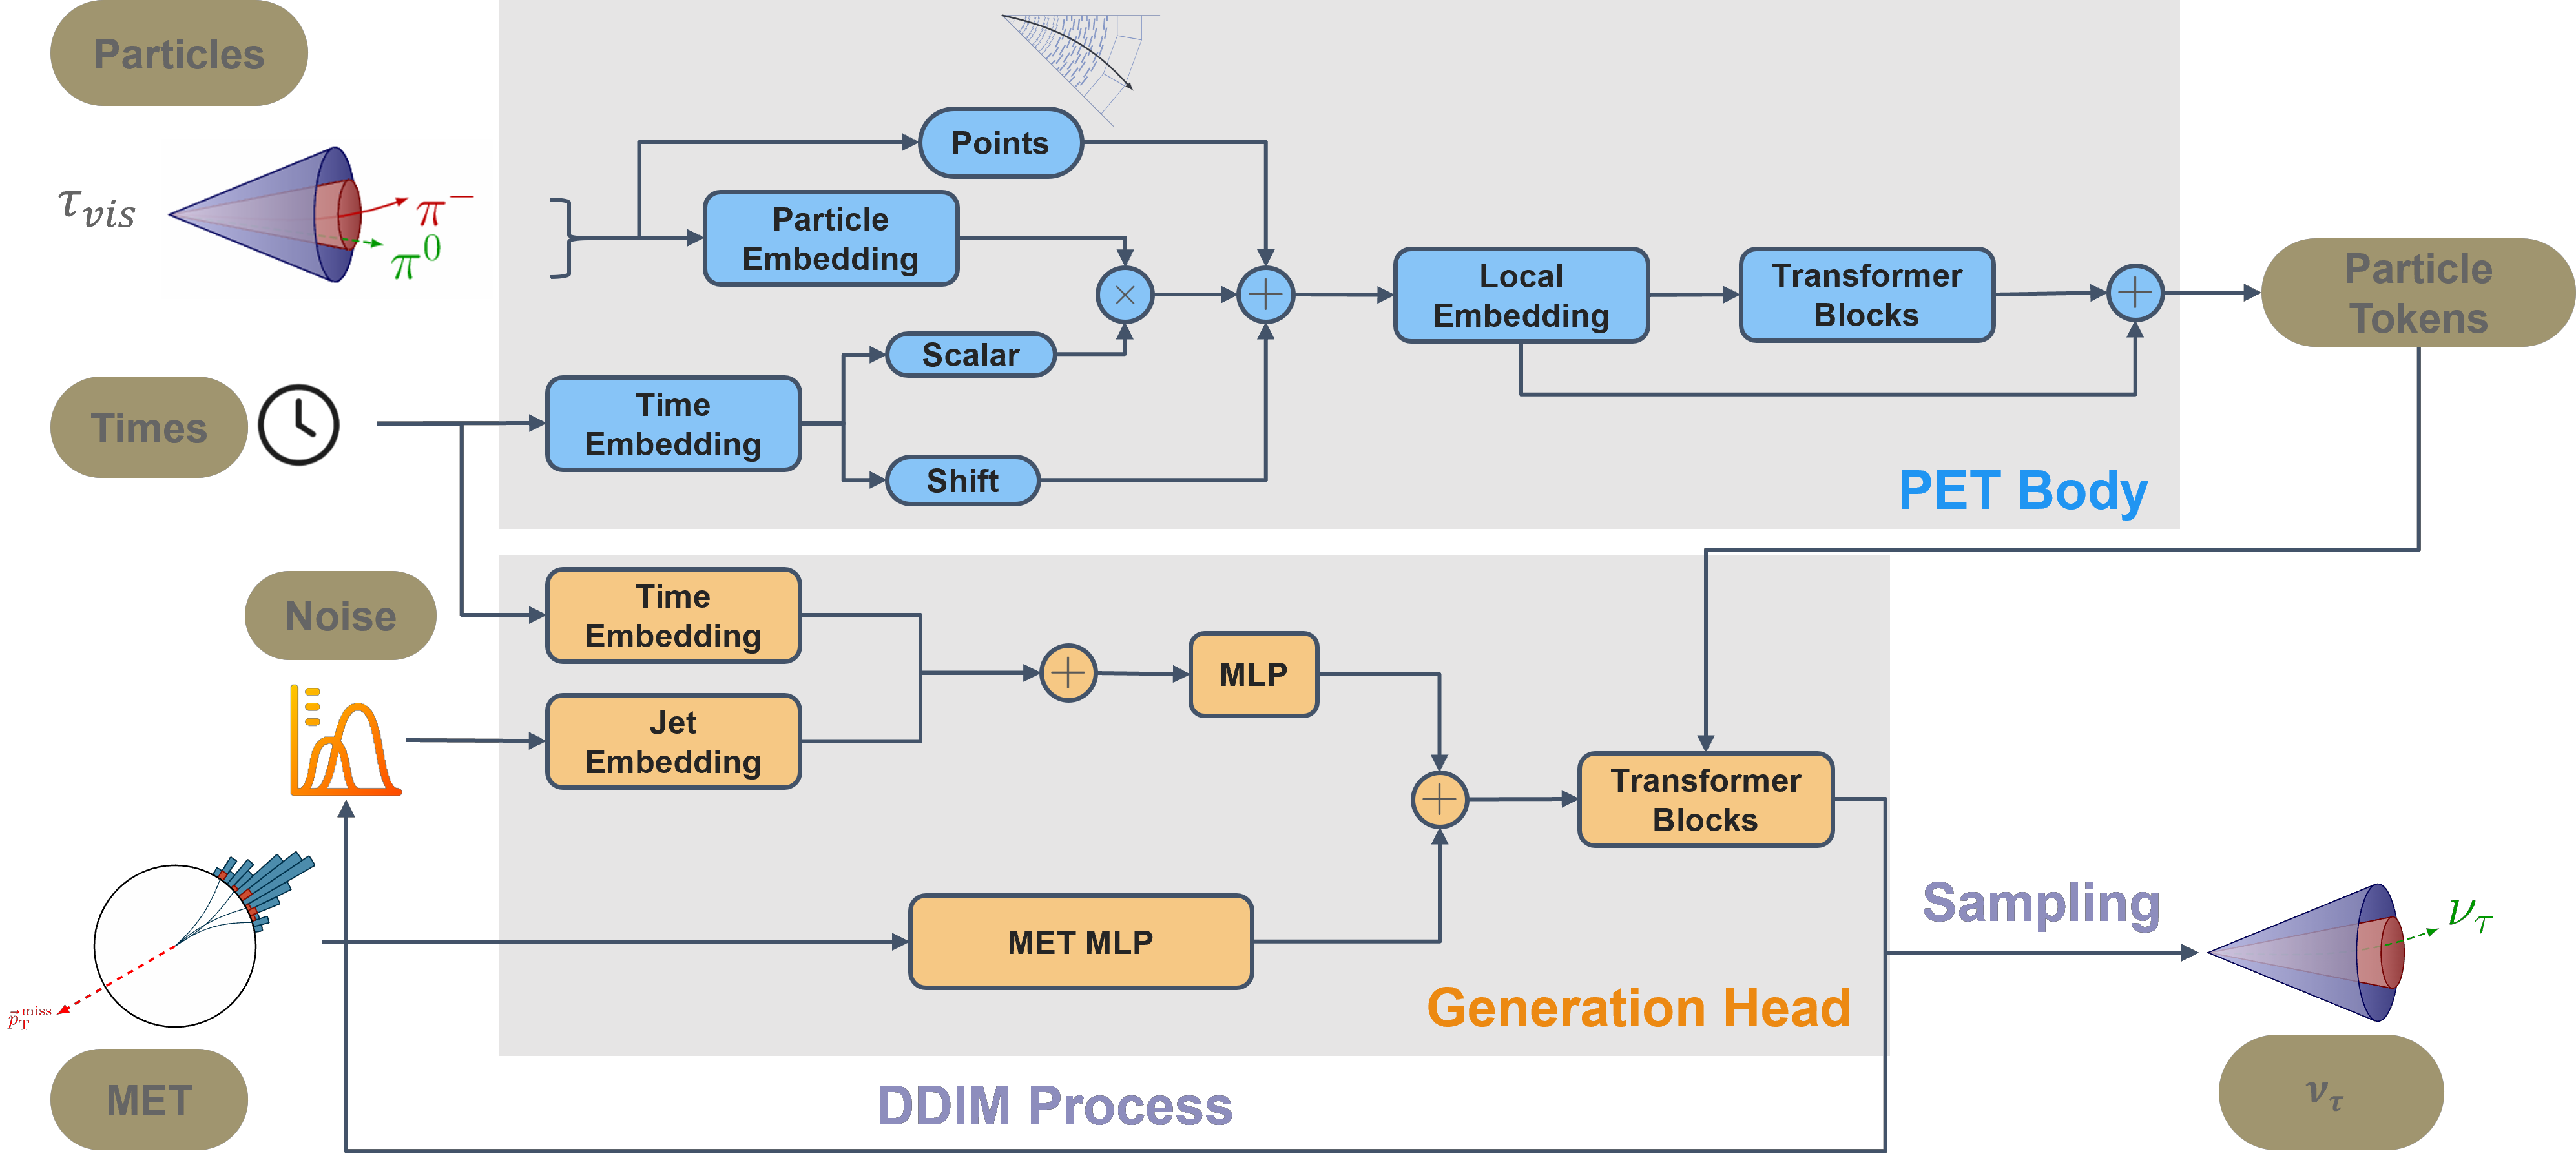
\includegraphics[height=6.0cm]{figures/omni}
\caption{OmniLearn生成模型架构}
\label{fig:OmniLearn}
\end{figure}

\section{模型训练过程}
\label{sec:threepfour}

本研究的数据集采用与文献[7]相同的蒙特卡洛模拟方法取得：使用MadGraph 5[22]在13 TeV的质心能量下生成$pp \to \tau \bar{\tau} X$事件，并要求末态的不变质量大于20 GeV；随后利用MadGraph中的taudecay\_UFO模型使$\tau $子经过五个衰变道包括$\pi \pi $、$\pi \rho$ 、$\rho \rho$ 、$l \pi$ 和$l \rho$进行衰变，其中每个衰变道对应$10^7$个事例；再将这些事件中的粒子输入Pythia 8[23]进行底层事件模拟、部分子簇射和强子化处理；最后使用Delphes[24]默认配置模拟探测器响应。此外，研究基于探测器的旋转对称性采用了一种数据增强策略：质心参考系下，将每个模拟事件在横向平面上随机旋转某一角度。该策略使得训练样本数提高了约50倍。

在训练开始前，将数据集的80\%划为训练集，剩余的20\%则用于检查训练过程是否出现过拟合等问题。学习率通过预热和余弦衰减的方式进行动态调整，初始值设置为$1.2 \times 10^{-4}$ ；优化器使用Lion优化器，超参数分别为$ \beta_1=0.95$，$ \beta_2=0.99$。

去噪扩散概率模型的采样步数设置为200步。在中微子动量的重建过程中，针对每个事件共生成10个候选的中微子，并随机挑选其中的1个用于后续处理。相比于对动量取平均的方法，可以验证随机挑选这一策略所取得的结果更接近原始值。